% Appendices file. here, cover all topics related to thesis.


% PERFORMANCE METRICS ==========================================================
\section{Performance Metrics}
The concept of verifying accuracy in a statistical estimate is covered in [xx source], and some of this information is covered briefly below. In the field of image recognition, one particularly interesting metric is "Intersection over Union", also referred to as IOU or Jaccard Index. From this metric, precision and recall may then be calculated. Precision and recall are fundamental in obtaining more abstracted metrics such as Average Precision and mean Average Precision (mAP), which are how different networks are compared. The following information is primarily taken from the well-known PASCAL VOC (visual objects classes) Challenge \cite{everingham_pascal_2010} and "An Introduction to Information Retrieval" by \cite{manning_introduction_2008}.

\subsection{Defining a Result}
The first step in measuring performance is categorizing what a result may be. With a visual task such as object classification, there are 4 possible outcomes, as shown below. In general, there may be a True Positive, False Positive, True Negative, or False Negative. In practice, True Negatives are not used, and the remaining three are used to varying degrees. Each is better clarified as such:
\begin{itemize} \itemsep=-.5em
	\item True Positive: Correctly detecting a true object
	\item False Positive: Incorrectly detecting something that isn't there
	\item False Negative: Incorrectly ignoring a true object
	\item True Negative: Correctly ignoring something that isn't there
\end{itemize}

\begin{figure}[h] % h = "approx here", {h,t,b}
	\centering
	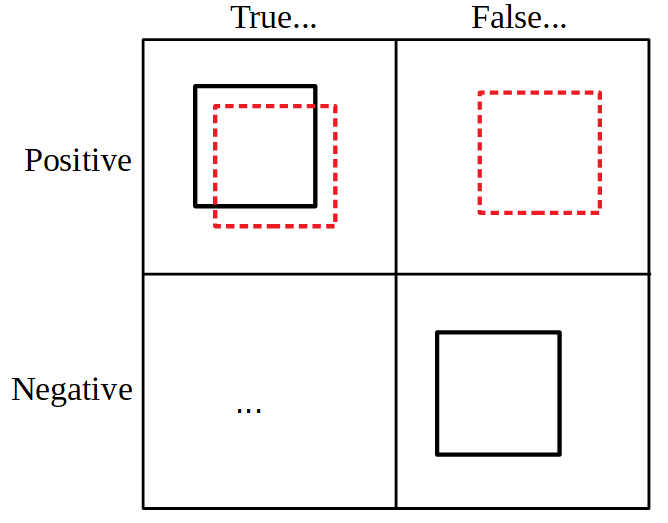
\includegraphics[width=.4\textwidth]{../media/tp_help.png}
	\caption{A visual representation of various outcomes, ground truths as solid black boxes and detections as dotted red boxes. True positives (TP) are a correct detection, FP's are a detection of no actual object, and FN's are a lack of detection of an actual object.}
	\label{tp_help} %label goes last
\end{figure}

To actually classify a result in one of these categories, computer vision depends on using the overlap of a given bounding box estimate with a bounding box ground truth. If the overlap is above some threshold, the estimate is said to be a true positive. In some metrics, two estimates overlapping the same ground truth will only count the larger overlap, or the more confident estimate. Overlap is formally known as Intersection over Union, or IOU value.

\subsection{Intersection Over Union}
In image recognition, as well as other spatially-based tasks, accuracy is needed in various forms to know "how well" a prediction overlaps, or matches, the ground truth. If, for example, an object-detection algorithm predicts the location of a car in a photo, one would like to know if such an estimate has any value, ideally with as few parameters as possible.

In light of this, Intersection Over Union encompasses all relevant aspects of rating the overlap of two geometric shapes (e.g. rectangles) while enabling an intuive, non binary scoring of an estimate. IOU is calculated as the ratio of two bounding regions' intersection over their union, as the name states. Visually, this looks something like the below in Figure \ref{iou_img}. Uniquely, the calculation of area and intersection for image boundaries is inclusive of the bounds, meaning that the length of a given difference must have ``+1" added to it. This is explained in the example below.

\begin{figure}[ht] % h = "approx here", {h,t,b}
    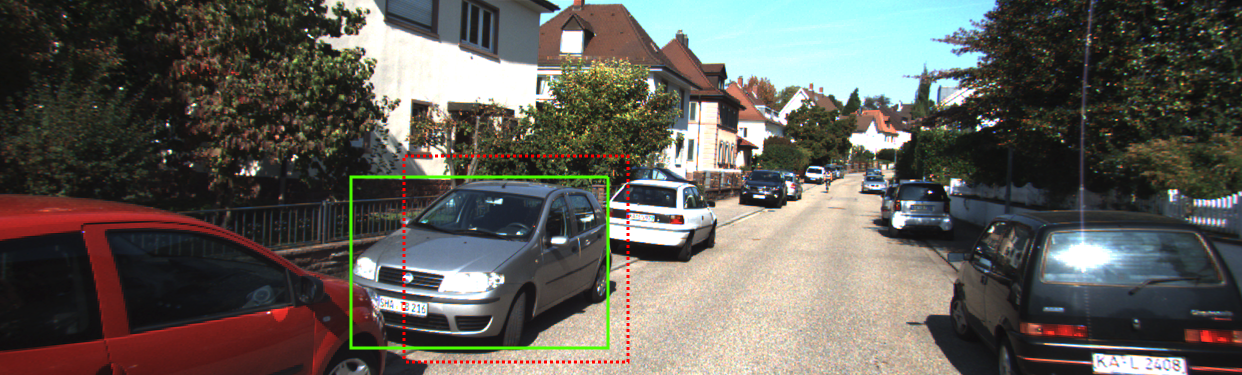
\includegraphics[width=1\textwidth]{../media/iou_img.png}
    \caption{Example of ground truth bounding box (solid green) and prediction bounding box (dashed red). In this image, the overlap between the green and red regions is the intersection, while the combined area is the union. The IOU of the two boxes is 0.64. Image index: 8.}
    \label{iou_img} %label goes last
\end{figure}

In order to formally calculate IOU, a generalized form may be generated to apply to n-dimensions. The generalized mathematical equation is simply as follows. Given a region A and a region B: 
\begin{equation}
IOU = \frac{|A\cap B|}{|A\cup B|} = \frac{|A\cap B|}{|A|+|B|- |A\cap B|}
\end{equation}

To assist in understanding IOU, a code snippet as well as an example are presented.

All aspects of calculating the IOU (including area and intersection) are broken up into multiple pieces, but presented together below. For n-dimensions, the code (presented here in python) is as follows: 


KJG190618: NEED TO RE-PASTE IN THIS CODE!!! XX
\begin{figure}[H]
\setstretch{0.84} % want code to be nice and compact
\begin{lstlisting}
import numpy as np

def extent(box,inclusive=False):
    '''
    Return the size or "extent" (length, area, volume, etc) of a given box in
        n-dimensions.
    INPUTS:
        box: n-dimensional bounds, format [x1,y1,z1, .. ,x2,y2,z2, ..]
        inclusive: boolean. add 1 unit to calculation, such as for image area
    OUTPUT:
        extent: size of box bounds, scalar float.
    NOTE:
    Internal convention: [Nx2] array,
        | x1 x2 |
        | y1 y2 |
        | z1 z2 |
        | .. .. |
    '''
    o= 1 if(inclusive) else 0 # add '1' if inclusive is true
    b=np.array(box).reshape((2,-1)).T # now in internal convention
    return np.product([i[1]-i[0]+o for i in b])
def intersection(box1,box2,inclusive=False):
    '''
    Return the size / "extent" of intersection between two bounds of
        n-dimension. Internal convention follows same as "extent" function.
    INPUTS:
        box1,box2: n-dimensional bounds, format [x1,y1,z1, .. ,x2,y2,z2, ..]
    OUTPUT:
        intersection: size of overlapping bounds, scalar float.
    '''
    o= 1 if(inclusive) else 0 # add '1' if inclusive is true
    b1=np.array(box1).reshape((2,-1)).T
    b2=np.array(box2).reshape((2,-1)).T # internal convention
    c=np.stack((b1,b2),2)
    # for each dimension, get (min(upperbound)-max(lowerbound)) and get product
    val=1
    for i in range(len(b1)):
        ans=np.min(c[i,1,:])-np.max(c[i,0,:])
        val*=max(ans,0) # if have negative dimension, have no intersection
    return val

def IOU(b1,b2,inclusive=False):
    '''
    Return generalized intersection over union for two bounding boxes of
        matching n-dimension.
    INPUTS:
        b1,b2: n-dimensional bounding boxes, format [x1,y1,z1, .. ,x2,y2,z2, ..]
    OUTPUT:
        iou: intersection over union, scalar float, range [0,1].
    '''
    inter = intersection(b1,b2,inclusive)
    union = extent(b1,inclusive)+extent(b2,inclusive)-inter
    return inter / union

\end{lstlisting}
\onehalfspacing % set line spacing back to normal
\caption{Python implementation of generalized IOU calculation.}
\label{code_iou}
\end{figure}

\subsubsection{Example: IOU of a Ground Truth and Prediction Label}
Suppose there is an image, as given below, where there is a ground truth label `gt' and a prediction label `pred' with 2D bounding boxes formatted as \texttt{[x1,y1,x2,y2]}, all units in pixels. To determine the IOU of the image, the calculations are listed below. Because boxes represent pixel values, remember to add "1" to each dimension.



\def \pxpx {\; [px^2]}
\def \Asub #1{A\textsubscript{#1}}
\begin{enumerate}\itemsep=-0.5em

\item Find area of each bounding box: \\ $\Asub{gt} = (x2-x1+1)*(y2-y1+1) = 16,335 \pxpx $ , $ \Asub{pr} = 12905 \pxpx $

\item Find overlapping area, e.g. intersection (see \ref{code_iou} for more info): $I = 11455 \pxpx $

\item Calculate IOU: $\frac{I}{\Asub{gt} + \Asub{pr} - I} = 0.644 $
\end{enumerate}

\begin{figure}[h] % h = "approx here", {h,t,b}
    \centering
    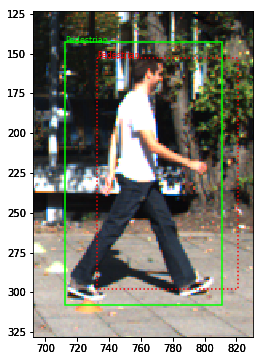
\includegraphics[width=.4\textwidth]{../media/iou_example.png}
    \caption{IOU calculation example. Ground truth (green solid) has BB: [712,143,810,307]. Prediction (red dotted) has BB: [732,153,820,297]. IOU is 0.644.}
    \label{iou_example} %label goes last
\end{figure}


\subsection{Precision \& Recall}
Once all detections have been tallied and placed into their correct categories, their precision and recall may be calculated. In information retrieval, precision is defined as "the fraction of retrieved documents that are relevant", and recall is defined as "the fraction of relevant documents that are retrieved". Reworded for object detection: precision is the number of correct predictions divided by the total number of predictions, and recall is the number of correct predictions divided by the total number of possible answers. These two are also given as equations in terms of true positives and so on. 

\begin{equation}
Precision = \frac{TruePositives}{TruePositives + FalsePositives}
\end{equation}

\begin{equation}
Recall = \frac{TruePositives}{TruePositives + FalseNegatives}
\end{equation}

In practice, the precision and recall of each detection is generated procedurally as each detection is compared to ...

KJG190618: NEED TO PERSONALLY RUN THROUGH A SIMPLE EXAMPLE OF PRECISION / RECALL, AND PUT THIS INTO YOUR PYTHON SANDBOX XX

% ABOUT THE KITTI DATASET ======================================================
\newpage
\section{About the KITTI Dataset}

\subsection{Introduction}
To better understand the actual data that is being worked on, the KITTI dataset will be explained in-depth here. KITTI itself is a combination of "KIT" (Karlsruhe Institute of Technology) and "TTI" (Toyota Technical Institute, Chicago), the two cooperating institutions on the project. The very first thing to know about the KITTI dataset is that it is actually a set of datasets, each dataset specialized for some specific AI task. This means that there are some number of evaluation tasks / benchmarks, and a not-necessarily-unique dataset is used to enable completion of that task. The individual tasks are listed below with a brief description: 

\begin{itemize}\itemsep=-0.5em 
    \item Stereo, Optical Flow, Sceneflow (2012 \& 2015): An older (2012) and updated (2015) task comprised of 200 training and 200 test scenes. Each scene consists of a left and right image as well as a "multi-view extension".
    \item Depth Completion / Estimation: A task comprised of about 93 thousand scenes containing RGB images and lidar scans.
    \item Visual Odometry / SLAM: 11 training and 11 testing stereo sequences with relevant grayscale, color, lidar, and ground truth poses.
    \item 2D / 3D / Bird's Eye View (BEV) Detection: 7481 training and 7518 test scenes with relevant color images, temporally preceding images, and lidar
    \item Single-/Multi- Object Tracking: An older (single) and in-development (multi) task consisting of multiple training and test sequences with relevant image, lidar, and GPS/IMU data. 
    \item Road / Lane Detection: Around 289 training and 290 test images used for detecting various road scenes, containing image and lidar information.
    \item Semantic / Instance Segmentation: A task comprised of a set of stereo images like the Stereo task, but containing pixel-level localization of each class. 
\end{itemize}

Each evaluation task also brings with it a "dev kit" (a set of files that explain some of the technical information as well as helpful code), relevant camera / sensor calibration data of some kind, as well as some kind of ground truth label / file for each scene to assist with training. It should be noted that raw data of each dataset is available as well, but these are often unused and only kept as original source files for transparency. Below in Figure \ref{kitti_samples} is an image summary taken from the various tasks to give a quick and simple overview of the variety of datasets.

\begin{figure}[H]
    \centering
    \subfigure[Stereo, Optical Flow, Sceneflow (2015)]{
        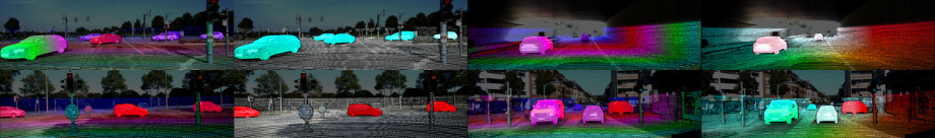
\includegraphics[width=1\linewidth]{../media/kitti_1_stereo.png}}
    \subfigure[Depth Completion, Depth Evaluation (2017)]{
        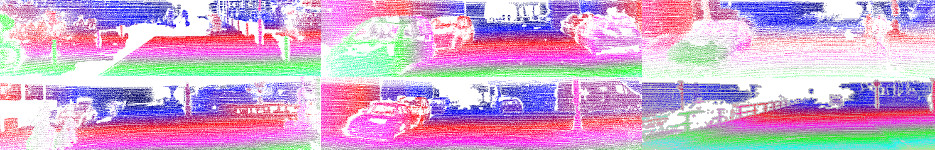
\includegraphics[width=1\linewidth]{../media/kitti_2_depth.png}}
    \subfigure[Visual Odometry / SLAM (2012)]{
        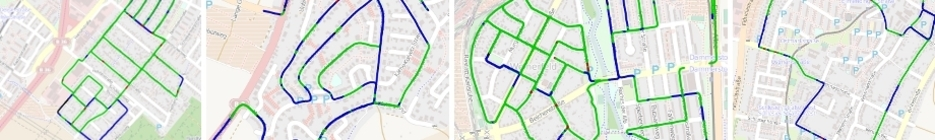
\includegraphics[width=1\linewidth]{../media/kitti_3_odom.png}}
    \subfigure[2D (2012), 3D (2017), Bird's Eye View (2017) Object Detection]{
        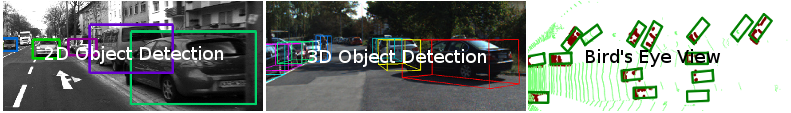
\includegraphics[width=1\linewidth]{../media/kitti_4_objdet.png}}
    \subfigure[Single Object(2012), Multi-Object (ongoing) Tracking]{
        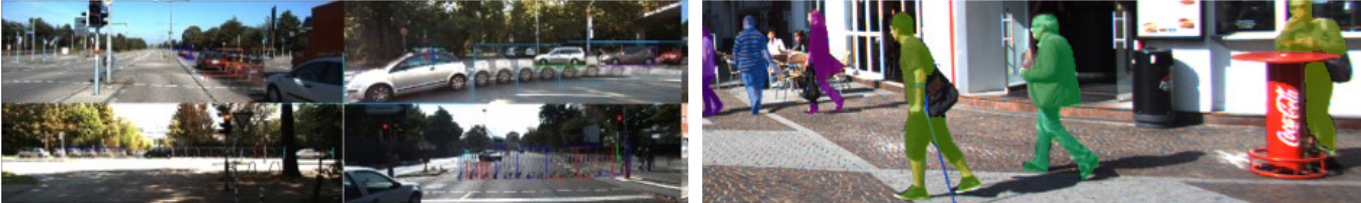
\includegraphics[width=1\linewidth]{../media/kitti_5_track.png}}
    \subfigure[Road / Lane Detection (2013)]{
        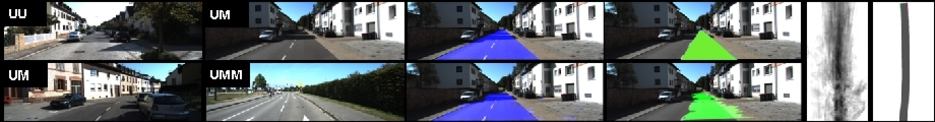
\includegraphics[width=1\linewidth]{../media/kitti_6_road.png}}
    \subfigure[Semantic and Instance Segmentation (2015)]{
        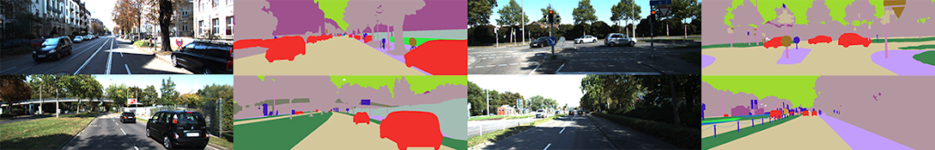
\includegraphics[width=1\linewidth]{../media/kitti_7_seg.png}}
    \caption{xx add more detail}
    \label{kitti_samples}
\end{figure}

Each task is associated with one or more papers published by KIT and TTI, but these will not all be listed here. Instead, we shall now explain two datasets, especially the most relevant one: the KITTI object detection dataset, referred to as the KITTI dataset.

\subsection{The Stereo Dataset}
The stereo dataset, specifically 2015, will be briefly covered to describe its merits as well as why it presented overlap issues with the object detection dataset. What makes the stereo dataset important is that it is the dataset that was initially used to finetune the Pyramid Stereo Matching network and also the dataset used to help it achieve such a high position in the stereo benchmark. 

The dataset itself is made up primarily of 200 training scenes and 200 testing scenes. The training scenes contain ground truth disparity maps, while the testing scenes do not and are used for final evaluation and submission to the benchmark website. For the project, only the training scenes were used. Each training scene is comprised of a left-hand side (LHS) color image, a RHS color image, a calibration file (containing transformation and other matrices), and a ground truth disparity file. There is also an available "multi-view extension", containing 20 extra frames per scene, but this was not used. Figure \ref{stereo_sample} below shows all relevant data in a single sample scene: the left and right images, as well as a disparity map ground truth.

\begin{figure}[H]
    \centering
    \subfigure[LHS image]{
        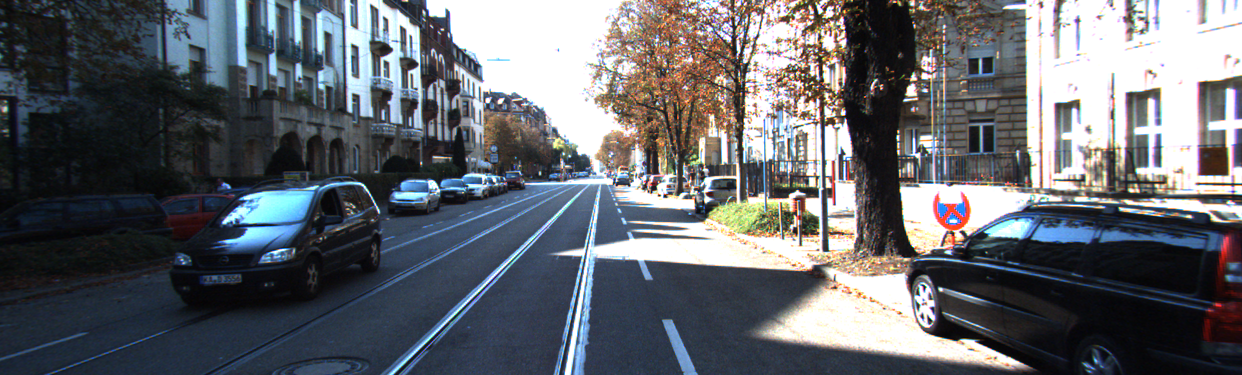
\includegraphics[width=0.487\linewidth]{../media/stereo_LHS_000000_10.png}}
    \subfigure[RHS image]{
        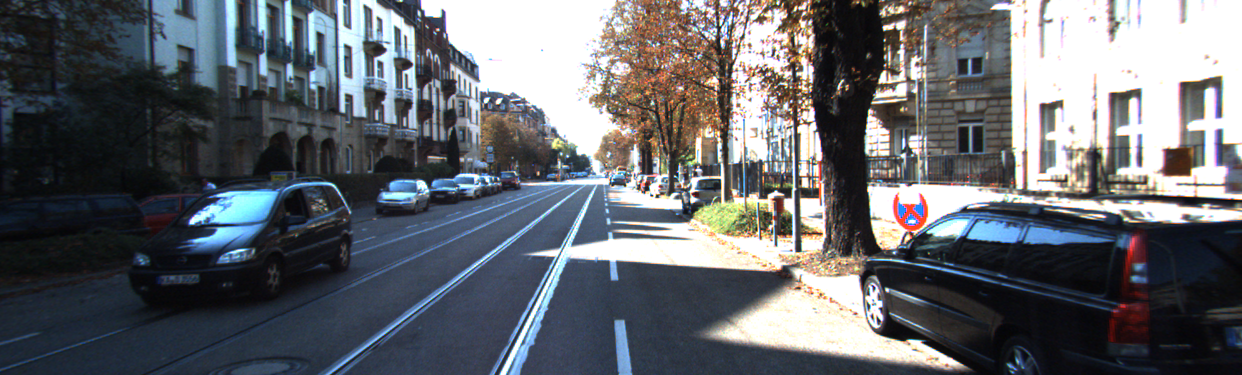
\includegraphics[width=0.487\linewidth]{../media/stereo_RHS_000000_10.png}}
    \subfigure[Ground truth disparity map with a viridis colormap. The value range for the original ground truth file may lie anywhere from 1 to 33,000 or a little higher. Disparity is a measure of how far apart one pixel is relative to its matching pixel in another location. ]{
        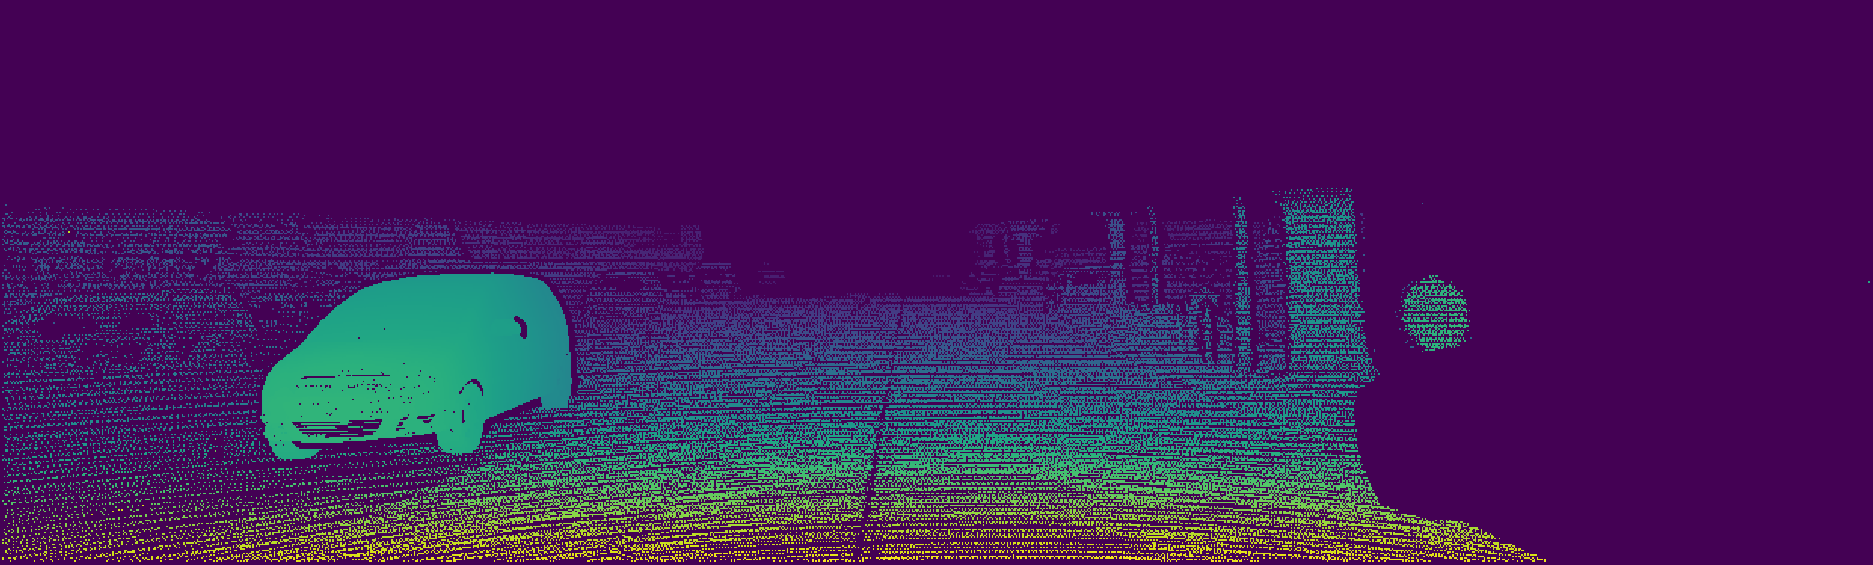
\includegraphics[width=1\linewidth]{../media/stereo_GTdisp_000000_10.png}}
    \caption{Sample scene from stereo dataset. Index 000000\_10}
    \label{stereo_sample}
\end{figure}

The ground truth labels were generated by a "semi-automatic" process, as described by Menze and Geiger: the process was to "extract disparity maps directly from the 3D information int he laser scans and fit geometrically accurate CAD models to moving 3D point clouds" \cite{Menze_2015_CVPR}. This explains several things about the ground truth disparity map in Figure \ref{stereo_sample}(c): the image is generally sparse, has no sample values above a certain horizontal line, and has a high density of pixels in the region where a car is outlined.

Ultimately, however, this dataset was not used for the primary reason described by \cite{wang_pseudo-lidar_2019}: there was an unacceptable amount of overlap, also known as data leakage, between the stereo dataset training data and the similar but unrelated object detection dataset. Figure \ref{similarity_stereo_objdet}, shown in Section 3, gives an example of a scene in the stereo dataset nearly matches a scene in the object detection dataset.

\subsubsection{The Object Detection Dataset \& Statistics}
The Object Detection dataset is the primary source of sensor data and media for this project, including PSMnet once it was determined that the stereo dataset had too much similarity with this dataset. The Object Detection dataset is comprised of 7481 training scenes and 7518 testing scenes. The testing scenes were ignored for the purposes of this project, since they are unlabeled for KITTI benchmarking. Each scene in the training dataset contains a LHS (left-hand side) image, RHS image, lidar data, calibration data, and ground truth labels. An example of the images and lidar are given below in Figure \ref{objdet_sample}. 

\begin{figure}[H]
    \centering
    \subfigure[LHS image]{
        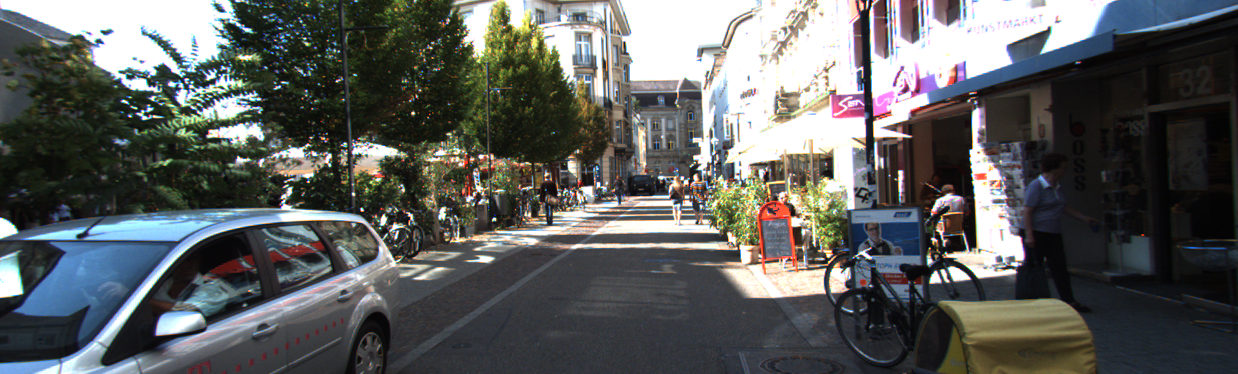
\includegraphics[width=0.487\linewidth]{../media/objdet_LHS_000015.png}}
    \subfigure[RHS image]{
        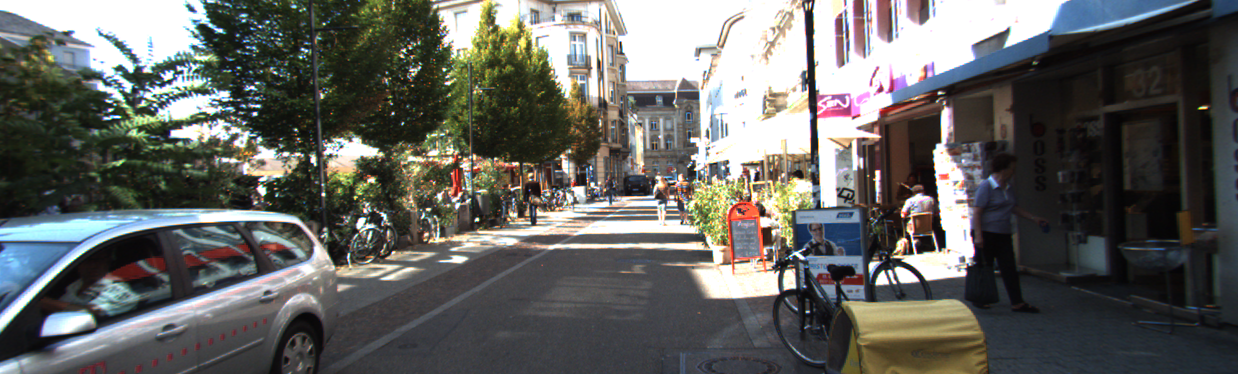
\includegraphics[width=0.487\linewidth]{../media/objdet_RHS_000015.png}}
    \subfigure[Velodyne lidar points projected onto image plane. Gray background for ease of viewing. Individual points use viridis colormap.]{
        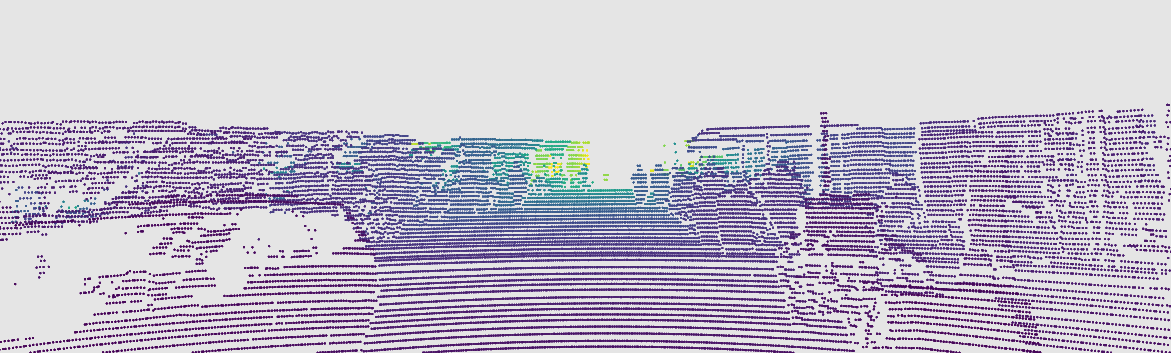
\includegraphics[width=1\linewidth]{../media/objdet_lidar_000015.png}}
    \caption{Sample scene from object detection dataset. Index 000015}
    \label{objdet_sample}
\end{figure}

In addition to the above lidar projection, the point cloud may be better visualized with an isometric view, rather than one from the camera's perspective. This is provided below, with 3D bounding boxes provided for reference.

\begin{figure}[H]
    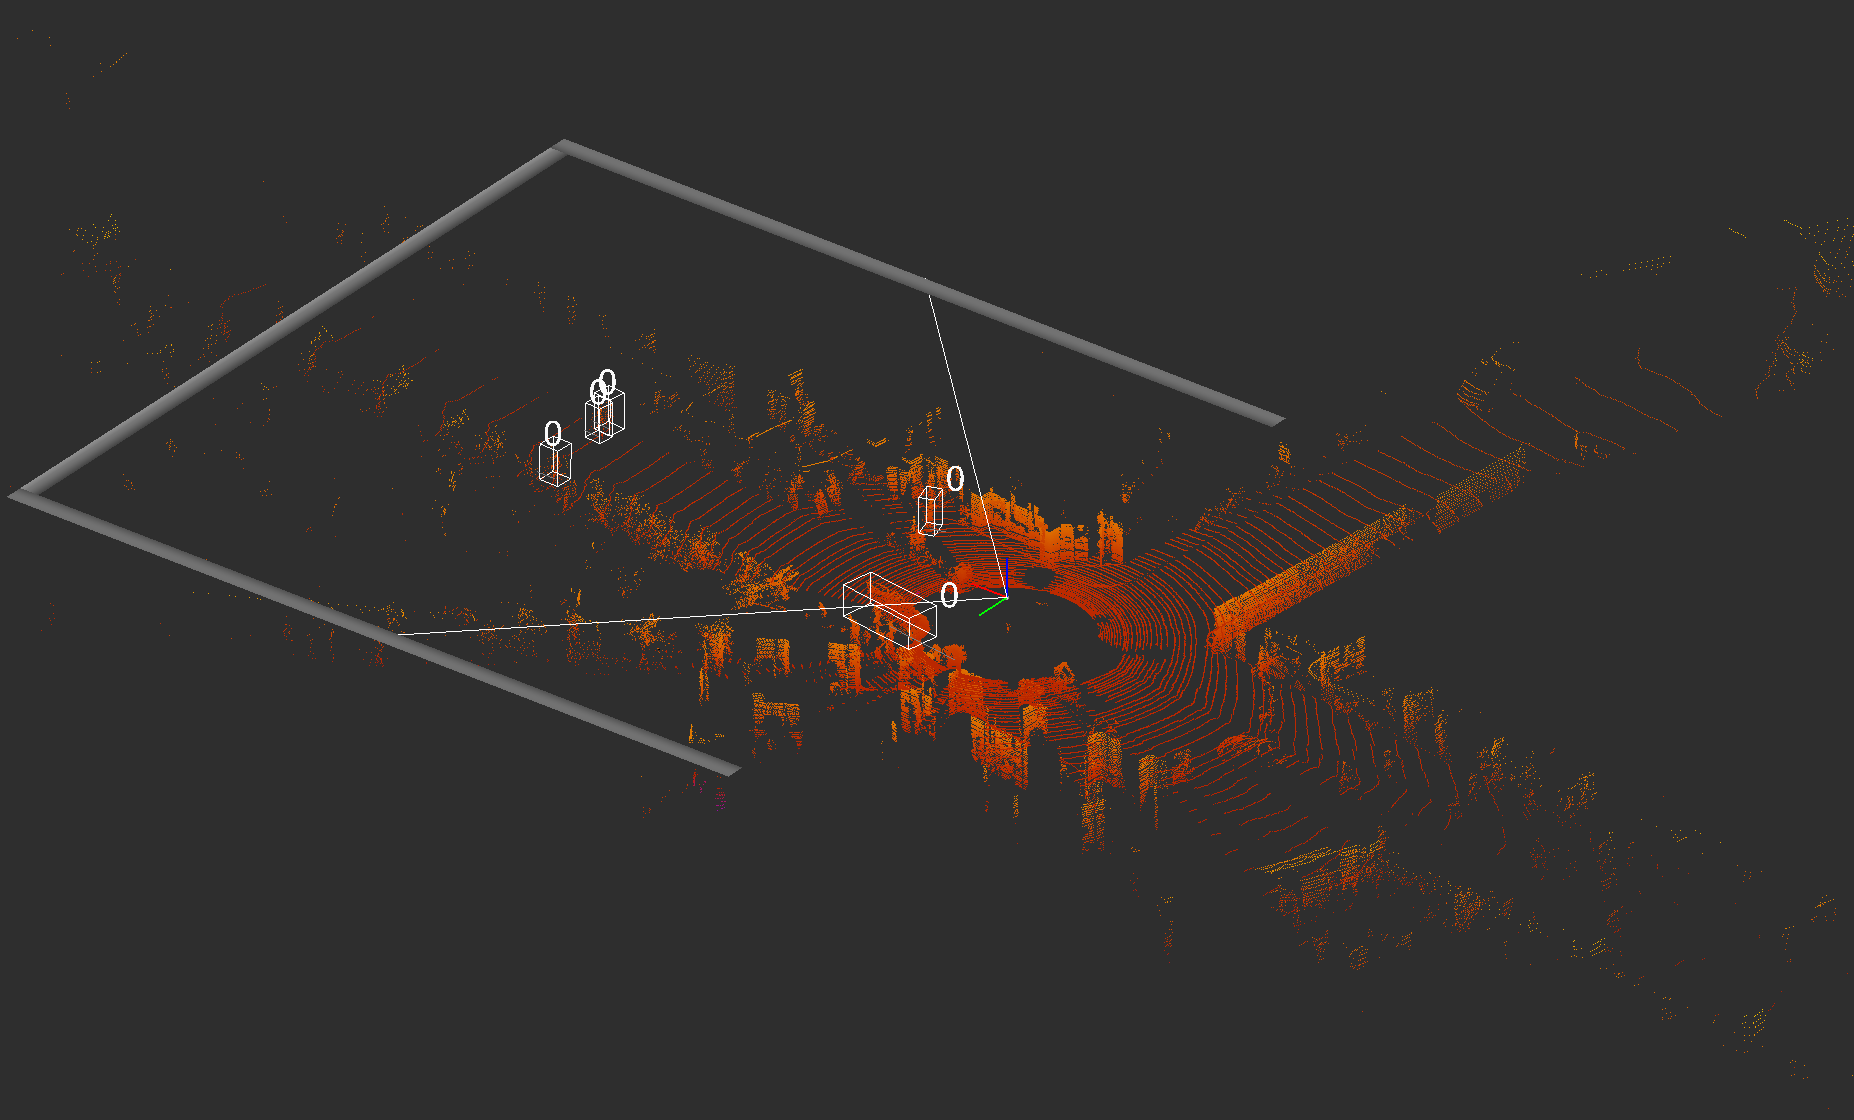
\includegraphics[width=1\linewidth]{../media/objdet_lidar_BEV_000015.png}
    \caption{Lidar pointcloud, alternate view. 3D bounding boxes are included as well as the horizontal field of view (white angled lines leading away from coordinate system origin). Index 000015}
    \label{objdet_lidar_sample}
\end{figure}

\def \DEG{$^{\circ}$} % Don't want to import extra package for no reason right now.

As is immediately obvious above in Figure \ref{objdet_lidar_sample} and from knowledge of the hardware itself, a lidar scan is capable of capturing points surrounding the sensor in a 360\DEG horizontal view. However, because of the nature of a typical color camera, points that are outside the camera's field of view are filtered out. 

Ground truth labels are simply text files that contain an array of information about each instance of an object in the scene. An example line is given below in table xx. 


\begin{table}[h]
\centering
\caption{KITTI object detection sample label from a given scene. Index 000015}
\begin{tabular}{|c|c|c|c|c|c|c|c|c|c|c|c|c|c|c|}
\hline
Class & Trun & Occl & Obs  & BBx1  & BBy1   & BBx2   & BBy2   & HT & WD & DP & Cx    & Cy   & Cz   & Roty \\
\hline
Car   & 0.89       & 0         & 2.29 & 0.00  & 194.70 & 414.71 & 373.00 & 1.57   & 1.67  & 4.14  & -2.75 & 1.70 & 4.10 & 1.72 \\

\hline
\end{tabular}
\label{Mathematical Symbols}
\end{table}


Beyond a few samples of the dataset, some statistics about the dataset can be found in both the accompanying paper as well as by looking through the dataset itself. When observing only the training data, the count of each class can be described. 







% SAMPLE =======================================================================
\newpage
\section{Sample Appendix}
TextHere

\begin{figure}[h] % h = "approx here", {h,t,b}
    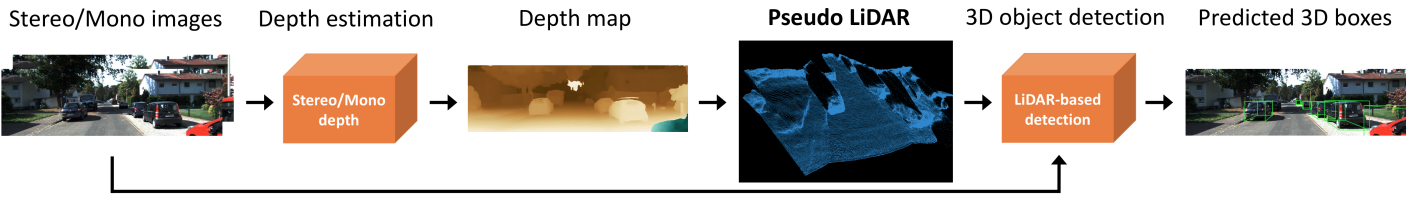
\includegraphics[width=1\textwidth]{../media/wang_pipeline.png}
    \caption{texthere}
    \label{delme_figure} %label goes last
\end{figure}


\begin{figure}[h] %h=here,t=top,b=bottom,H=exactlyHere
\setstretch{0.84} % want code to be nice and compact
% note: optional line numbers argument
\begin{lstlisting}[numbers=left]
def pyt(a,b):
    return (a**2+b**2)**0.5
\end{lstlisting}
\onehalfspacing % set line spacing back to normal
\caption{Python implementation of generalized IOU calculation.}
\label{delme_code} % label goes last
\end{figure}

%\begin{enumerate}\itemsep=-0.5em
%	\item one
%	\item two
%	\item three
%\end{enumerate}
